\documentclass[12pt, a4paper, titlepage]{article}
\usepackage[a4paper, total={6in, 8in}]{geometry}
\usepackage[skip=0.7em, indent=1.8em]{parskip}
\usepackage{microtype}

% Images
\usepackage{graphicx}
\usepackage{float}
\usepackage{caption}
\usepackage{subcaption}

% Citations
\usepackage[
    backend=biber,
    sorting=none,
    style=numeric-comp,
]{biblatex}
\setlength\bibitemsep{\baselineskip}
\addbibresource{cit.bib}

% PDF outline, hyperlinks, properties
\usepackage[
    bookmarks,
    pdfborder={0 0 0},
    pdftitle={History of Biology \& Genetics},
    pdfauthor={Subhaditya Nath},
    pdfkeywords=LS1201,
]{hyperref}

% Font
\usepackage[rmlining]{merriweather}

% Headings
\usepackage{titlesec}
\usepackage{relsize}
\usepackage{xcolor}
\titlelabel{\textcolor{lightgray}{\smaller[3]\normalfont\thetitle.} }

% Titlepage
\title{
    History of Biology \& Genetics \\
    \small From the earliest to the latest concepts
}
\author{Subhaditya Nath \\ 22MS145}
\date{\vskip 1em
    Spring 2023 \\
    \small LS1201
}

% Document
\begin{document}
\maketitle

% Table of Contents (Summary)
\renewcommand*\contentsname{Summary}
\addtocontents{toc}{\protect\thispagestyle{empty}}
\pagenumbering{gobble}
\tableofcontents
\newpage
\pagenumbering{arabic}



\section{Introduction}
The study of living creatures and their vital activities is known as biology. It is the scientific study of living beings, including their structure, function, growth, evolution, and interactions with the environment. It covers a wide range of issues, from molecular and cellular biology to environmental complexity and the diversity of life on Earth. Biology is the study of the features and processes that define living creatures, such as their structure, metabolism, reproduction, genetics, and adaptation. It also investigates how creatures interact with one another and with their surroundings, looking into ecological interactions, behaviour, and the impact of human activities on the natural world.

William Bateson invented the term Genetics to describe the scientific study of genes and heredity; how specific attributes or traits are handed down from parents to offspring as a result of variations in DNA sequence. Humans recognised that one of the reasons of variety was hidden in sexual reproduction as early as 8000-1000 B.C. They took advantage of inherent variability in plant and animal populations to selectively propagate and select species with desirable features. A more-than-6000-year-old Babylonian tablet, for example, depicts horse pedigrees and possible inherited features. Other Assyrian carvings depict date palm tree cross-pollination. Selective breeding of cattle, horses, and dogs existed long before Mendel. Genetics history can be separated into two eras --  Pre-Mendelian and Post-Mendelian.


\section{Cell theory}
\subsection{Discovery of cells}
In 1665, Robert Hooke was the first person to find the cell. He wrote about it in his book \textit{Micrographia}. In this book, he wrote about 60 detailed notes of different things seen through a coarse compound microscope.

One of the observations was of thin slices of bottle cork. Hooke found a lot of small holes that he called ``cells." This comes from the Latin word \textit{Cella}, which means ``a small room" like the ones monks live in, and \textit{Cellulae}, which means ``a honeycomb cell with six sides."

\begin{figure}[H]
    \centering
    \caption{Robert Hooke's drawings from \textit{Micrographia}}
    \begin{subfigure}{0.45\textwidth}
        \centering
        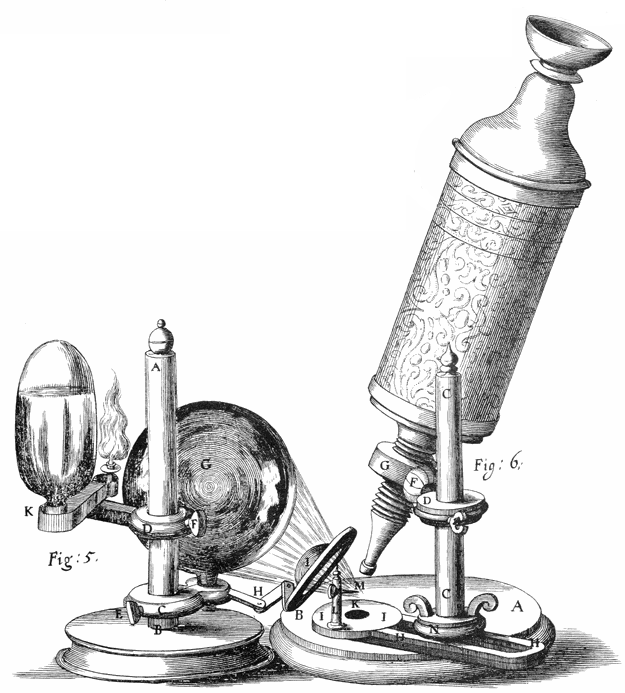
\includegraphics[scale=0.25]{img/hooke-scope.png}
        \caption{Microscope}
    \end{subfigure}
    \begin{subfigure}{0.45\textwidth}
        \centering
        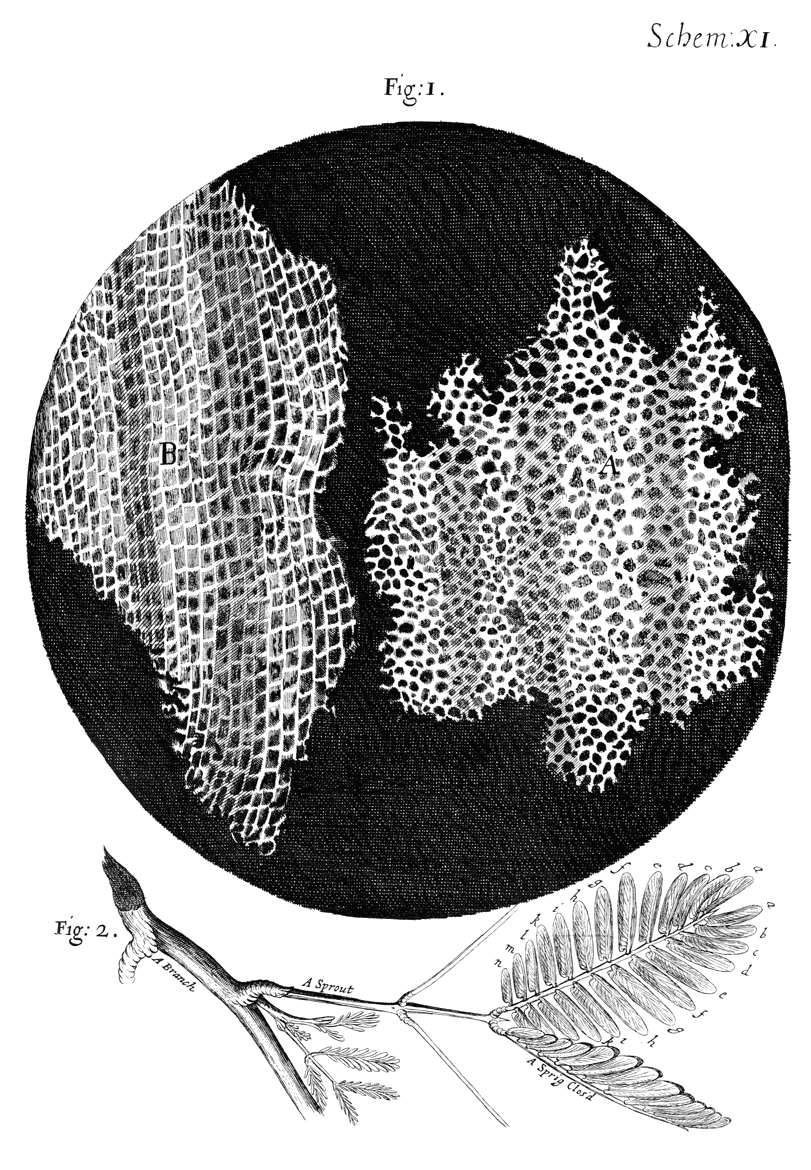
\includegraphics[scale=0.15]{img/hooke-draw.png}
        \caption{Structure of cork}
    \end{subfigure}
\end{figure}

However, Hooke did not know their real structure or function. Since he was unable to see that there were other internal components to the cells he was observing, he did not think that the ``cellulae" were alive.\supercite{gest2004}

\subsection{Cell theory}
Credits for developing cell theory goes to Theodor Schwann and Matthias Jakob Schleiden.\supercite{sharp1921}



\newpage
\printbibliography
\end{document}
